%\section{Grundlagen, Stand der Forschung}
% infromieren what quarter- / halfwaveplate und polarizer are
% - Halfwaveplates:
%   Rotate Polarisation
% - Quarterwaveplates:
%   Turn linear to circular polarization

\section{Grundlagen}
In diesem Kapitel wird das notwendige Wissen für die vorliegende Arbeit vermittelt. Es werden Grundlagen über die Administration bezüglich Softwareentwicklung als auch Methoden zum Programmieren von Programmen für die Entwicklung einer Software beschrieben.\\

\subsection{Agile Software-Engineering}
Der Ansatz der agilen oder auch inkrementelle Softwareentwicklung wurde aus Gründen der Zusammenarbeit mit dem Kunden (Empfänger und Nutzer des Softwareproduktes) entwickelt. Durch die inkrementelle Auslieferung an den Kunden, hat dieser die Möglichkeit neue Funktionen spontan anzubringen und wurde aus diesem Grund ausgewählt. Daneben ist die inkrementelle Softwareentwicklung geeignet für kleine Software und kleinere, flexible Kunden. Die Anforderungen können zu jedem Zeitpunkt abgeändert oder angepasst werden. [6]

Wurden die Anforderungen im Vorhinein definiert und werden im Verlauf des Projekts nicht abgeändert, resultiert eine eher vermischte Methode, die sogenannte plangesteuerte und agile Entwicklung. Dabei werden Iterationsschritte lediglich in den einzelnen Projektphasen zugelassen und verändern nicht die gesamte Struktur des Projektes. Jedoch ist es trotzdem möglich Änderungen in der Anforderungsspezifikation vorzunehmen, wenn dies in der Entwurfs- und Implementierungsphase detektiert wird. In grösseren Projekten werden die Phasen Entwurf und Implementierung getrennt. In kleineren Projekten wie diesem, verschmelzen diese Phasen und alle anderen Aktivitäten werden in diesen Prozess integriert. Programme sollen mit einer guten Softwarepraxis entwickelt werden, damit diese Wiederverwendung finden und diese gut zu Unterhalten sind. Dazu sollen sie für den Ersteller und andere Programmierer:innen nachvollziehbar sein.
Verbesserungen können in der Regel schnell implementiert werden. Dazu fällt das akribische Dokumentieren und Planen im Vorfeld weg. Dies hat für den Empfänger und für die Entwickler einen grossen Vorteil. [6] % S. 214

\begin{figure}[H]
    \centering
    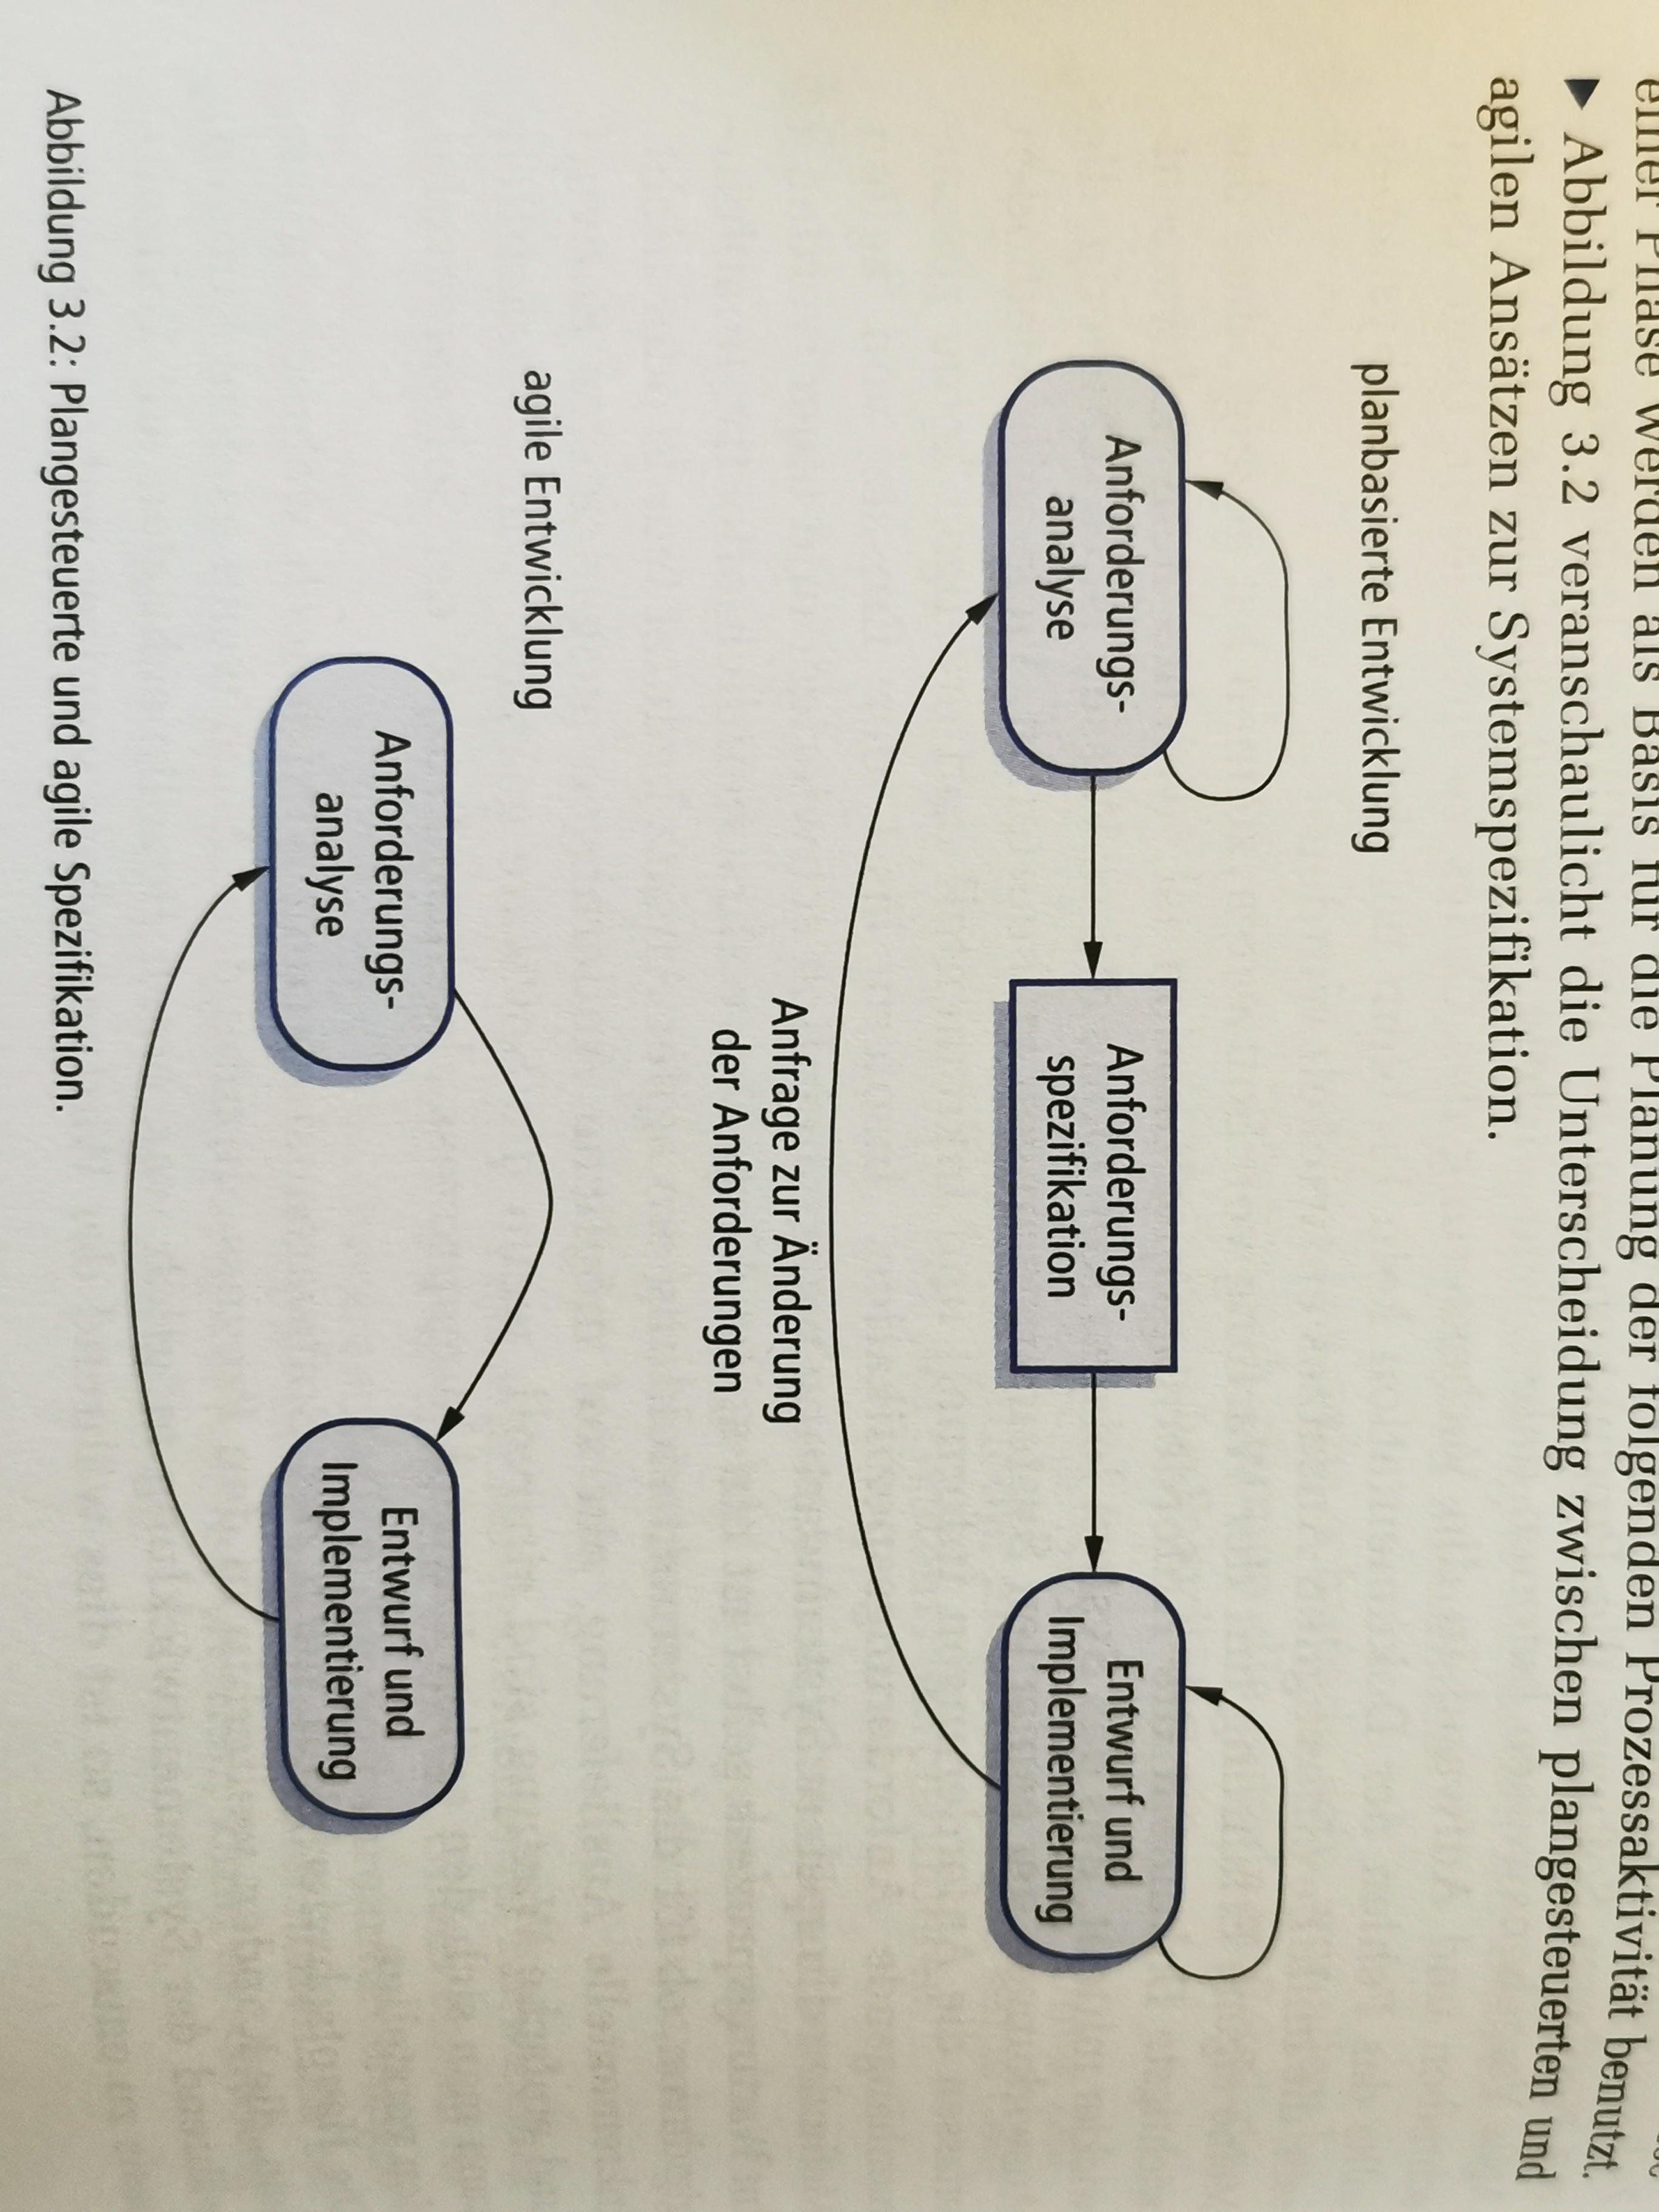
\includegraphics[scale=0.08, angle=90, clip]{98_images/plangesteuerte_agile_development.jpg}
    \caption{Die Graphik zeigt die Agile-Plangesteuerte Methode. [6]}
    \label{fig:agile_method}
\end{figure}

% \textit{Commercial Off-the-Shelf, COTS}: bereits fertiges System, das mit wenigen Anpassungen einsatzbereit ist (Meerstetter MeCom API) aber kostenlos erhältlich -->

\subsection{Wiederverwendbarkeit von Software - Objektorientiertes Programmieren}
Um die Software effizienter gestalten zu können, wurde wo dies möglich war auf die Wiederverwendbarkeit von Software dritter zugegriffen. So wurde z.B. die Kommunikation mit dem TEC-Kontroller erstellt. Den Quellcode für die Kommunikation mit dem TEC-Kontroller wurde von Meerstetter Engineering, der Hersteller Firma des TEC-Treibers zur Verfügung gestellt.\\
Für die graphische Benutzeroberfläche wurde das Framework von \textit{Customtkinter} und \textit{Tkinter} verwendet. Damit lassen sich graphische Oberflächen einfacher erstellen. Neben den Frameworks wurden auch sogenannte Bibliotheken verwendet wie \textit{Numpy} und  \textit{Pandas} für das hantieren mit Vektoren und Tabellen.\\

Zusätzlich wurde soweit es ging objektorientiertes Programmieren eingesetzt. Dies vereinfacht die Übersicht des Programmcodes massiv. Dabei werden Teile des Programmcodes, die wiederholt vorkommen und eine gleiche bis ähnliche Struktur aufweisen, mit immer der gleichen Vorlage erstellt. Für kleinere Abweichungen können der Vorlage Parameter mitgegeben werden, die das zu erstellende Objekt leicht abändert.

\subsection{Entwurfsmuster - Design Patterns}
Für die Programmierung der Steuerung wurde ein sogenanntes Entwurfsmuster, auch \textit{Design Pattern} genannt verwendet. Entwurfsmuster sind verallgemeinerte vordefinierte Programmiermethodiken und Softwarearchitekturen, die für gewisse Fälle in der Softwareentwicklung erdacht wurden. Sie sind dazu da wiederkehrende Probleme in der Softwareentwicklung mit einer geeigneten spezifischen Methode zu lösen. Daneben ermöglichen sie eine einfache Handhabung mit Daten, Infrastrukturen, Anzeigen und der Erweiterung und Abänderung des Programmcodes zu jeder Zeit und ohne anderen Code drastisch zu verändern. Unter den Entwurfsmuster gibt es wiederum verschieden Kategorien, die die Einsatzgebiete der Entwurfsmuster beschreiben. Grundsätzlich jedoch werden die Beschreibungen der Muster in vier Hauptgruppen unterteilt. Der Name, das Problem, die Lösung und die Konsequenz beim Verwenden des Musters. Mit dieser Beschreibung kann für das vorliegende Problem das geeignetste Muster gefunden werden. $[7]$

% [https://medium.com/@amirm.lavasani/design-patterns-in-python-a-series-f502b7804ae5]

\subsection{Parallelität / Gleichzeitigkeit im Programm}
\label{concurrency}
Weil ein Prozessor in einem Rechner bzw. in einem Prozessor Informationen nur seriell verarbeiten kann, ist es nicht möglich mit einem synchronen Programm die geforderten Aufgaben abzuarbeiten. Der inaktive Prozess würde nicht flüssig laufen, die Aufgabe würde somit nicht zeitgerecht ausgeführt. Zeigen kann sich dieser Effekt, wenn zum Beispiel die Anzeige einfriert und somit nicht mehr bedienbar ist. Das Lesen der Daten des TEC-Controllers und des Pumpdiodentreibers und das Anzeigen der Daten in der Benutzeroberfläche sind zwei Prozesse. Die Aufgaben für die Steuerung müssen also asynchron oder parallel abgearbeitet werden. Um dieses Problem zu bewältigen, gibt es drei Programmiermethodiken, die ein Programm in verschiedene \textit{Pfade oder Aufgaben} aufteilt. Asynchrones programmieren mit der Bibliothek \textit{asyncio}, \textit{Threading} oder die Multiprozessorprogrammierung, wobei asynchrone Abläufe und \textit{Threading} sehr ähnlich sind. In den Illustrationen gezeigt werden die Unterschiede der Methoden.

\begin{figure}[H]
    \centering
    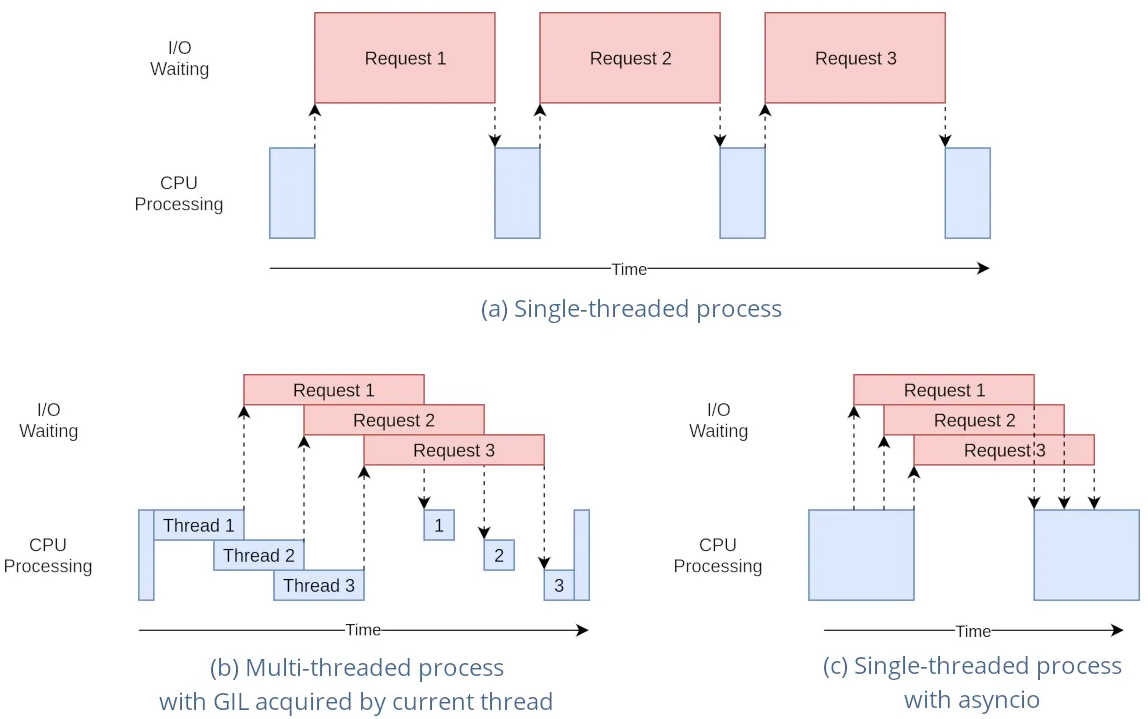
\includegraphics[scale=0.4]{98_images/thread_vs_async_vs_single.png}  % https://blog.stackademic.com/multithreading-vs-asynchronous-programming-f015c6b676d0  % Bild
    \caption{Die Unterschiedlichen Arbeitsweisen der verschiedenen Programmiertechniken. Bei der Multiprozessormethode ist der Zugriff auf den geteilten Speicher nicht gezeigt.}
    \label{fig:multi_threading_async}
\end{figure}

\begin{table}[H]
    \centering
    \begin{tabular}{l|c|c|c}
         \multicolumn{1}{c|}{$-$}&   \textbf{Asynchron}& \textbf{Threading}& \textbf{Multiprozessor}\\
         \hline
         Standardbibliothek&        Ja&                 Ja&                 Ja\\
         Komplexität&               Fortgeschritten&    Fortgeschritten&    Komplex\\
         Nutzen&                    Ja&                 Ja&                 Ja\\
         Erfahrung&                 Nein&               Ja&                 Nein
    \end{tabular}
    \caption{In der Tabelle sind verschiedene Methoden, um Programme asynchron oder parallel ablaufen zu lassen aufgelistet.}
    \label{tab:async_threading_multiprocessor}
\end{table}

Bei der asynchronen Methode und beim \textit{Threading} werden vom einen Prozess Aufgaben ausgeführt, wenn ein anderer Prozess eine Wartezeit durchläuft. Dies ist immer der Fall, wenn ein Prozess eine Brachzeit wechselt und  den Prozessor des Rechners nicht verwendet, dann kann ein anderer Prozess den Prozessor nutzen. Beim Multiprozessor werden die parallel auszuführenden Aufgaben auf verschiedene Prozessoren aufgeteilt, verhindern sich somit nicht direkt. Die Schwierigkeit jedoch ist die Datenintegrität zu gewährleisten. Alle getrennten Prozesse müssen zur richtigen Zeit mit der korrekten Datengrundlage arbeiten können. Woher weiss Prozess A, dass die Daten auf dem gemeinsam genutzten Speicher von Prozess B fertig verarbeitet sind? $-$ Neben anderen Herausforderung bei der Multiprozessor Programmierung, stellt dies die grösste Herausforderung dar. Aus den oben genannten Gründen wurde das \textit{Threading} gewählt. $[11]$

% https://medium.com/velotio-perspectives/an-introduction-to-asynchronous-programming-in-python-af0189a88bbb

\subsection{Serielle Kommunikationsschnittstelle - USB}
Für die Übertragung der Daten vom TEC-Kontroller wurde das USB Protokoll verwendet. Der TEC-Controller kann so direkt an den Raspberry PI angeschlossen werden und die API der Herstellerfirma Meerstetter, kann auch direkt verwendet werden. Diese Schnittstelle erwies sich währen der Test als stabil. Der Nachteil ist, dass wenn Parameter auf dem TEC -Kontroller geändert werden müssen, muss die Steuerung geöffnet werden.

% Und noch schnell die ganze Bibliographie zitieren:
\nocite{*}